% LaTeX source for textbook ``How to think like a computer scientist''
% Copyright (C) 1999  Allen B. Downey
% Copyright (C) 2009  Thomas Scheffler

\chapter{Iteration}

\section{More on assignments }
\index{assignment}
\index{statement!assignment}
\index{multiple assignment}
\index{self assignment}
\index{assignment!multiple}
\index{assignment!self}
\index{assignment!operator}
I haven't said much about it, but it is legal in C to
make more than one assignment to the same variable.  The
effect of the second assignment is to replace the old value
of the variable with a new value.

\begin{verbatim}
  int fred = 5;
  printf ("%i", fred);
  fred = 7;
  printf ("%i", fred);
\end{verbatim}
%
The output of this program is {\tt 57}, because the first
time we print {\tt fred} its value is 5, and the second time
its value is 7.

This kind of {\bf multiple assignment} is the reason I
described variables as a {\em container} for values.  When
you assign a value to a variable, you change the contents of
the container, as shown in the figure:

\vspace{0.1in}
\centerline{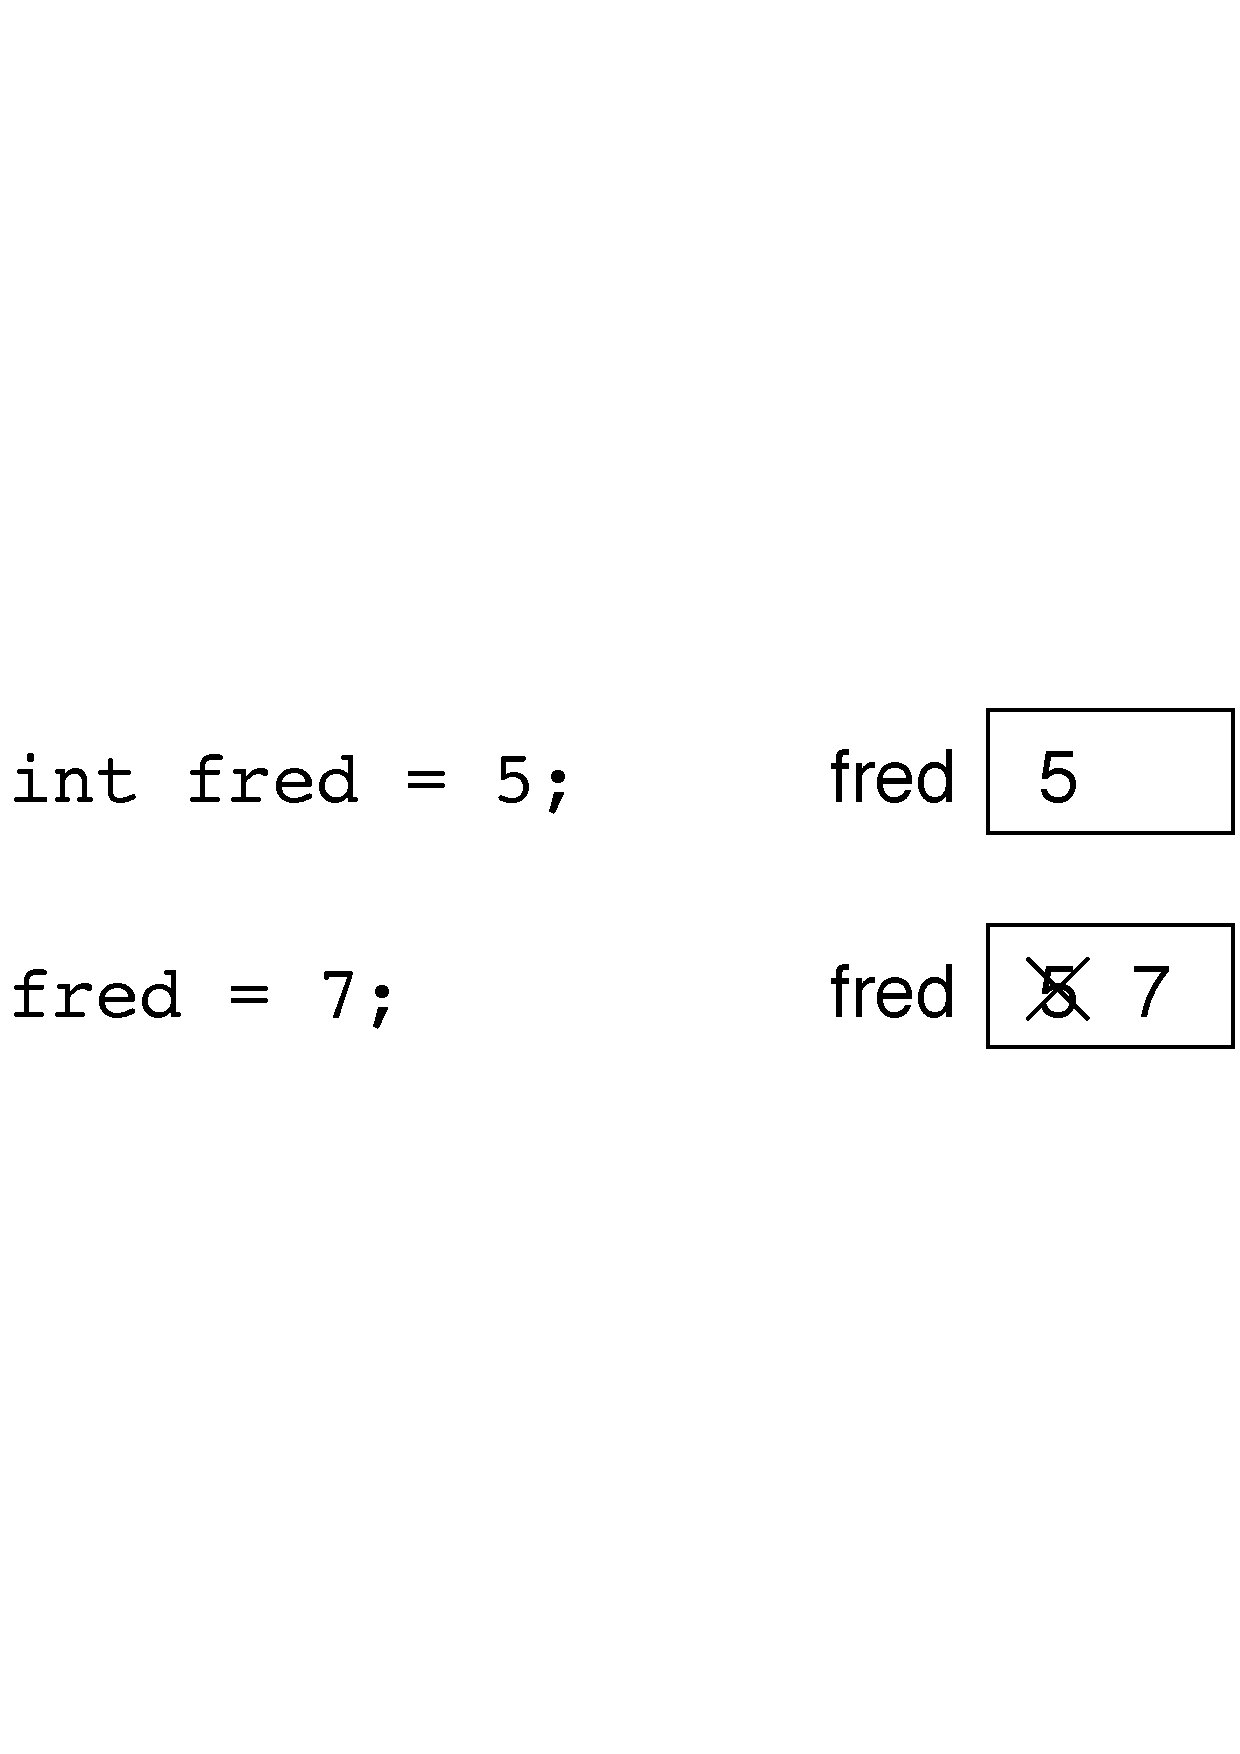
\includegraphics[height=1.8cm]{figs/assign2.pdf}}
\vspace{0.1in}

When there are multiple assignments to a variable, it is especially
important to distinguish between an assignment statement and a
statement of equality.  Because C uses the {\tt =} symbol for
assignment, it is tempting to interpret a statement like {\tt a = b}
as a statement of equality.  It is not! In many programming languages 
an alternate symbol is used
for assignment, such as {\tt <-} or {\tt :=}, in order to
avoid confusion.

First of all, equality is commutative, and assignment is not.
For example, in mathematics if $a = 7$ then $7 = a$.  But in
C the statement {\tt a = 7;} is legal, and {\tt 7 = a;}
is not.

Furthermore, in mathematics, a statement of equality is true
for all time.  If $a = b$ now, then $a$ will always equal $b$.
In C, an assignment statement can make two variables equal,
but they don't have to stay that way!

\begin{verbatim}
  int a = 5;
  int b = a;     /* a and b no have the same value*/
  a = 3;         /* a and b are no longer have the same value */
\end{verbatim}
%
The third line changes the value of {\tt a} but it does not
change the value of {\tt b}, and so they are no longer equal.

The ability to make multiple assignments to a variable means we can {\bf self assign} variables:

\begin{verbatim}
	int a = 5;  
	a = a + 1;       
\end{verbatim}
%
Assignment has the lowest precedent. 
This means that all other operations in the expression are evaluated before the assignment. 
In the first line code {\tt a} is initialized with a value of 5. In the second line, 
the expression  to the right of the assignment operator ($=$) is evaluated first. 
Since {\tt a} has the value 5, {\tt a + 1}  results in the value 6.
Finally we assign the result of 6 to {\tt a}..

\index{self assignment!operator}
\index{operator!self assignment}

Self assignment is actually very common. In fact, C has operators specifically for this task.

 \begin{verbatim}
 	int x = 3;
 	x += 2;  /* means x = x + 2 */      
 	x *= 4;  /* means x = x * 4  */      
 	x -= 6;  /* means x = x - 6  */      
 	x /= 6;  /* means x = x / 6   */    
 	x %=2 /* means x = x % 2 */  
 	
 \end{verbatim}
 %
 
\section{Iteration}
\index{iteration}

One of the things computers are often used for is the automation
of repetitive tasks.  Repeating identical or similar tasks without
making errors is something that computers do well and people do
poorly.

In section \ref{recursion} we have seen programs that use {\bf recursion} to perform
repetition, such as {\tt PrintLines()} and {\tt Countdown()}. 
I now want to introduce a new
type of repetition, that is called {\bf iteration}, and C provides
several language features that make it easier to write repetetive
programs.

The two features we are going to look at are the {\tt while}
statement and the {\tt for} statement.

\section{The {\tt while} statement}
\index{statement!while}
\index{while statement}

Using a {\tt while} statement, we can rewrite {\tt Countdown()}:

\begin{verbatim}
  void Countdown (int n) 
  {
      while (n > 0) 
      {
          printf ("%i\n", n);
          n = n-1;
      }
      printf ("Blastoff!\n");
  }
\end{verbatim}
%
You can almost read a {\tt while} statement as if it were
English.  What this means is, ``While {\tt n} is greater than
zero, continue displaying the value of {\tt n} and then reducing
the value of {\tt n} by 1.  When you get to zero, output the
word `Blastoff!'''

More formally, the flow of execution for a {\tt while} statement
is as follows:

\begin{enumerate}

\item Evaluate the condition in parentheses, yielding {\tt true}
or {\tt false}.

\item If the condition is false, exit the {\tt while} statement
and continue execution at the next statement.

\item If the condition is true, execute each of the statements
between the curly-brackets, and then go back to step 1.

\end{enumerate}

This type of flow is called a {\bf loop} because the third step loops
back around to the top.  Notice that if the condition is false the
first time through the loop, the statements inside the loop are
never executed.  The statements inside the loop are called
the {\bf body} of the loop.

\index{loop}
\index{loop!body}
\index{loop!infinite}
\index{body!loop}
\index{infinite loop}

The body of the loop should change the value of
one or more variables so that, eventually, the condition becomes
false and the loop terminates.  Otherwise the loop will repeat
forever, which is called an {\bf infinite loop}.  An endless
source of amusement for computer scientists is the observation
that the directions on shampoo, ``Lather, rinse, repeat,'' are
an infinite loop.

In the case of {\tt Countdown()}, we can prove that the loop
will terminate because we know that the value of {\tt n} is
finite, and we can see that the value of {\tt n} gets smaller
each time through the loop (each {\bf iteration}), so
eventually we have to get to zero.  In other cases it is not
so easy to tell:

\begin{verbatim}
  void Sequence (int n) 
  {
      while (n != 1) 
      {
          printf ("%i\n", n);
          if (n%2 == 0)       /* n is even */
          {          
              n = n / 2;
          } 
          else                /* n is odd */
          {                  
              n = n*3 + 1;
          }
      }
  }
\end{verbatim}
%
The condition for this loop is {\tt n != 1}, so the loop
will continue until {\tt n} is 1, which will make the condition
false.

At each iteration, the program outputs the value of {\tt n} and then
checks whether it is even or odd.  If it is even, the value of
{\tt n} is divided by two.  If it is odd, the value is replaced
by $3n+1$.  For example, if the starting value (the argument passed
to {\tt Sequence}) is 3, the resulting sequence is
3, 10, 5, 16, 8, 4, 2, 1.

Since {\tt n} sometimes increases and sometimes decreases, there is no
obvious proof that {\tt n} will ever reach 1, or that the program will
terminate.  For some particular values of {\tt n}, we can prove
termination.  For example, if the starting value is a power of two, then
the value of {\tt n} will be even every time through the loop, until
we get to 1.  The previous example ends with such a sequence,
starting with 16.

Particular values aside, the interesting question is whether
we can prove that this program terminates for {\em all} values of n.
So far, no one has been able to prove it {\em or} disprove it!

\section{Tables}
\index{table}
\index{logarithm}

One of the things loops are good for is generating
tabular data.  For example, before computers were readily available,
people had to calculate logarithms, sines and cosines, and other
common mathematical functions by hand.
To make that easier, there were books containing long tables
where you could find the values of various functions.
Creating these tables was slow and boring, and the result
tended to be full of errors.

When computers appeared on the scene, one of the initial reactions
was, ``This is great!  We can use the computers to generate the
tables, so there will be no errors.''  That turned out to be true
(mostly), but shortsighted.  Soon thereafter computers and
calculators were so pervasive that the tables became obsolete.

Well, almost.  It turns out that for some operations, computers
use tables of values to get an approximate answer, and then
perform computations to improve the approximation.  In some
cases, there have been errors in the underlying tables, most
famously in the table the original Intel Pentium used to perform
floating-point division.

\index{division!floating-point}

Although a ``log table'' is not as useful as it once was, it still
makes a good example of iteration.  The following program outputs a
sequence of values in the left column and their logarithms in the
right column:

\begin{verbatim}
  double x = 1.0;
  while (x < 10.0) 
  {
      printf ("%.0f\t%f\n", x ,log(x));
      x = x + 1.0;
  }
\end{verbatim}
%
The sequence \verb+\t+ represents a {\bf tab} character.
The sequence \verb+\n+ represents a newline character.  
They are so called \emph{escape sequences} which are used to encode
non-printable ASCII-characters.
Escape sequences can be included anywhere in a string, although in these examples
the sequence is the whole string.

A tab character causes the cursor to shift to the right until
it reaches one of the {\bf tab stops}, which are normally every
eight characters.  As we will see in a minute, tabs are useful
for making columns of text line up.
A newline character causes the cursor to move on to the next line.  
%Usually if a newline character appears by itself, I use {\tt endl}, but
%if it appears as part of a string, I use \verb+\n+.

The output of this program is:

\begin{verbatim}
   1      0.000000
   2      0.693147
   3      1.098612
   4      1.386294
   5      1.609438
   6      1.791759
   7      1.945910
   8      2.079442
   9      2.197225
\end{verbatim}
%
If these values seem odd, remember that the {\tt log()} function uses
base $e$.  Since powers of two are so important in computer science,
we often want to find logarithms with respect to base 2.  To do that,
we can use the following formula:

\[ \log_2 x = \frac {log_e x}{log_e 2} \]
%
Changing the output statement to

\begin{verbatim}
      printf ("%.0f\t%f\n", x, log(x) / log(2.0));
\end{verbatim}
%
yields:

\begin{verbatim}
    1      0.000000
    2      1.000000
    3      1.584963
    4      2.000000
    5      2.321928
    6      2.584963
    7      2.807355
    8      3.000000
    9      3.169925
\end{verbatim}
%
We can see that 1, 2, 4 and 8 are powers of two, because
their logarithms base 2 are round numbers.  If we wanted to find
the logarithms of other powers of two, we could modify the
program like this:

\begin{verbatim}
    double x = 1.0;
    while (x < 100.0) 
    {
        printf ("%.0f\t%.0f\n", x, log(x) / log(2.0));
        x = x * 2.0;
    }
\end{verbatim}
%
Now instead of adding something to {\tt x} each time through
the loop, which yields an arithmetic sequence, we multiply
{\tt x} by something, yielding a {\bf geometric} sequence.
The result is:

\begin{verbatim}
    1      0
    2      1
    4      2
    8      3
    16     4
    32     5
    64     6
\end{verbatim}
%
Because we are using tab characters between the columns, the
position of the second column does not depend on the number
of digits in the first column.

Log tables may not be useful any more, but for computer scientists,
knowing the powers of two is!  As an exercise, modify this program
so that it outputs the powers of two up to 65536
(that's $2^{16}$).  Print it out and memorize it.

\section{Two-dimensional tables}
\index{table!two-dimensional}

A two-dimensional table is a table where you choose a row and
a column and read the value at the intersection.  A multiplication
table is a good example.  Let's say you wanted to print a
multiplication table for the values from 1 to 6.

A good way to start is to write a simple loop that prints
the multiples of 2, all on one line.

\begin{verbatim}
    int i = 1;
    while (i <= 6) 
    {
        printf("%i   ", i*2);
        i = i + 1;
    }
    printf("\n");
\end{verbatim}
%
The first line initializes a variable named {\tt i}, which is
going to act as a counter, or {\bf loop variable}.  As the
loop executes, the value of {\tt i} increases from 1 to 6,
and then when {\tt i} is 7, the loop terminates.  Each
time through the loop, we print the value {\tt 2*i} followed
by three spaces.  By omitting the  \verb+\n+ from the
first output statement, we get 
all the output on a single line.

\index{loop variable}
\index{variable!loop}

The output of this program is:

\begin{verbatim}
    2   4   6   8   10   12
\end{verbatim}
%
So far, so good.  The next step is to {\bf encapsulate} and {\bf
generalize}.

\section {Encapsulation and generalization}

Encapsulation usually means taking a piece of code and wrapping it up
in a function, allowing you to take advantage of all the things functions
are good for.  We have seen two examples of encapsulation, when we
wrote {\tt PrintParity()} in Section~\ref{alternative} and {\tt
IsSingleDigit()} in Section~\ref{bool}.

Generalization means taking something specific, like printing
multiples of 2, and making it more general, like printing the
multiples of any integer.

\index{encapsulation}
\index{generalization}

Here's a function that encapsulates the loop from the previous
section and generalizes it to print multiples of {\tt n}.

\begin{verbatim}
    void PrintMultiples (int n)
    {
        int i = 1;
        while (i <= 6) 
        {
            printf("%i   ", i*n);
            i = i + 1;
        }
        printf("\n");
    }
\end{verbatim}
%
To encapsulate, all I had to do was add the first line,
which declares the name, parameter,
and return type.  To generalize, all I had to do was replace
the value 2 with the parameter {\tt n}.

If we call this function with the argument 2, we get the same
output as before.  With argument 3, the output is:

\begin{verbatim}
    3   6   9   12   15   18
\end{verbatim}
%
and with argument 4, the output is

\begin{verbatim}
    4   8   12   16   20   24 
\end{verbatim}
%
By now you can probably guess how we are going to print a
multiplication table: we'll call {\tt PrintMultiples()} repeatedly with
different arguments.  In fact, we are going to use another loop to
iterate through the rows.

\begin{verbatim}
    int i = 1;
    while (i <= 6) 
    {
        PrintMultiples (i);
        i = i + 1;
    }    
\end{verbatim}
%
First of all, notice how similar this loop is to the one inside {\tt
PrintMultiples()}.  I only replaced the call of the \texttt{printf()} function with 
the call of the \texttt{PrintMultiples()} function.

The output of this program is

\begin{verbatim}
    1   2   3   4   5   6   
    2   4   6   8   10   12   
    3   6   9   12   15   18   
    4   8   12   16   20   24   
    5   10   15   20   25   30   
    6   12   18   24   30   36   
\end{verbatim}
%
which is a (slightly sloppy) multiplication table.  If the
sloppiness bothers you, try replacing the spaces between
columns with tab characters and see what you get.

\section{Functions}
\index{function}

In the last section I mentioned ``all the things functions
are good for.''  About this time, you might be wondering
what exactly those things are.  Here are some of the reasons
functions are useful:

\begin{itemize}

\item By giving a name to a sequence of statements, you make
your program easier to read and debug.

\item Dividing a long program into functions allows you to
separate parts of the program, debug them in isolation, and
then compose them into a whole.

\item Functions facilitate both recursion and iteration.

\item Well-designed functions are often useful for many programs.
Once you write and debug one, you can reuse it.

\end{itemize}

\section{More encapsulation}
\index{encapsulation}
\index{program development!encapsulation}

To demonstrate encapsulation again, I'll take the code
from the previous section and wrap it up in a function:

\begin{verbatim}
    void PrintMultTable () 
    {
        int i = 1;
        while (i <= 6) 
        {
            PrintMultiples (i);
            i = i + 1;
        }
    }
\end{verbatim}
%
The process I am demonstrating is a common 
development plan.  You develop code gradually by adding
lines to {\tt main()} or someplace else, and then when you get
it working, you extract it and wrap it up in a function.

The reason this is useful is that you sometimes don't know
when you start writing exactly how to divide the program into
functions.  This approach lets you design as you go along.

\section{Local variables}

About this time, you might be wondering how we can use the same
variable {\tt i} in both {\tt PrintMultiples()} and {\tt
PrintMultTable()}.  Didn't I say that you can only declare a variable
once?  And doesn't it cause problems when one of the functions changes
the value of the variable?

The answer to both questions is ``no,'' because the {\tt i} in {\tt
PrintMultiples()} and the {\tt i} in {\tt PrintMultTable()} are
{\em not the same variable}.  They have the same name, but
they do not refer to the same storage location, and changing
the value of one of them has no effect on the other.

\index{local variable}
\index{variable!local}

Remember that variables that are declared inside a function definition
are local.  You cannot access a local variable from outside its
``home'' function, and you are free to have multiple variables with
the same name, as long as they are not in the same function.

The stack diagram for this program shows clearly that the
two variables named {\tt i} are not in the same storage location.
They can have different values, and changing one does not affect
the other.


\vspace{0.1in}
\centerline{\epsfig{figure=figs/stack4.pdf,width=6.5cm}}
\vspace{0.1in}
\index{stack diagram}
\index{diagram!stack}
%
Notice that the value of the parameter {\tt n} in
{\tt PrintMultiples()} has to be the same as the value
of {\tt i} in {\tt PrintMultTable()}.  On the other hand,
the value of {\tt i} in {\tt PrintMultiples()} goes
from 1 up to {\tt 6}.  In the diagram, it happens to be 3.
The next time through the loop it will be 4.

It is often a good idea to use different variable names in
different functions, to avoid confusion, but there are good
reasons to reuse names.  For example, it is common to
use the names {\tt i}, {\tt j} and {\tt k} as loop variables.
If you avoid using them in one function just because you
used them somewhere else, you will probably make the program
harder to read.

\index{loop variable}
\index{variable!loop}

%%
\section{More generalization}
\label{More generalization}
\index{generalization}

As another example of generalization, imagine you wanted
a program that would print a multiplication table of any
size, not just the 6x6 table.  You could add a parameter to
{\tt PrintMultTable()}:

\begin{verbatim}
    void PrintMultTable (int high) 
    {
        int i = 1;
        while (i <= high) 
        {
            PrintMultiples (i);
            i = i + 1;
        }
    }
\end{verbatim}
%
I replaced the value 6 with the parameter {\tt high}.  If I
call {\tt PrintMultTable()} with the argument 7, I get:

\begin{verbatim}
    1   2   3   4   5   6   
    2   4   6   8   10   12   
    3   6   9   12   15   18   
    4   8   12   16   20   24   
    5   10   15   20   25   30   
    6   12   18   24   30   36   
    7   14   21   28   35   42   
\end{verbatim}
%
which is fine, except that I probably want the table to
be square (same number of rows and columns), which means
I have to add another parameter to {\tt PrintMultiples()},
to specify how many columns the table should have.

Just to be annoying, I will also call this parameter {\tt high},
demonstrating that different functions can have parameters
with the same name (just like local variables):

\begin{verbatim}
  void PrintMultiples (int n, int high) 
  {
      int i = 1;
      while (i <= high) 
      {
          printf ("%i    ", n*i);
          i = i + 1;
      }    
      printf ("\n");
  }

  void PrintMultTable (int high) 
  {
      int i = 1;
      while (i <= high) 
      {
          PrintMultiples (i, high);
          i = i + 1;
      }
  }
\end{verbatim}
%
Notice that when I added a new parameter, I had to change the first
line of the function, and I also had to
change the place where the function is called in {\tt PrintMultTable()}.
As expected, this program generates a square 7x7 table:

\begin{verbatim}
    1   2   3   4   5   6   7   
    2   4   6   8   10   12   14   
    3   6   9   12   15   18   21   
    4   8   12   16   20   24   28   
    5   10   15   20   25   30   35   
    6   12   18   24   30   36   42   
    7   14   21   28   35   42   49
\end{verbatim}
%
When you generalize a function appropriately, you often find
that the resulting program has capabilities you did not intend.
For example, you might notice that the multiplication table
is symmetric, because $ab = ba$, so all the entries in the
table appear twice.  You could save ink by printing only
half the table.  To do that, you only have to change one
line of {\tt PrintMultTable()}.  Change

\begin{verbatim}
      PrintMultiples (i, high);
\end{verbatim}
%
to

\begin{verbatim}
      PrintMultiples (i, i);
\end{verbatim}
%
and you get:

\begin{verbatim}
    1   
    2   4   
    3   6   9   
    4   8   12   16   
    5   10   15   20   25   
    6   12   18   24   30   36   
    7   14   21   28   35   42   49  
\end{verbatim}
%
I'll leave it up to you to figure out how it works.

\section{Glossary}

\begin{description}

\item[loop:]  A statement that executes repeatedly while a
condition is true or until some condition is satisfied.

\item[infinite loop:]  A loop whose condition is always true.

\item[body:]  The statements inside the loop.

\item[iteration:]  One pass through (execution of) the body
of the loop, including the evaluation of the condition.

\item[tab:] A special character, written as \verb+\t+ in C,
that causes the cursor to move to the next tab stop on the
current line.

\item[encapsulate:]  To divide a large complex program into
components (like functions) and isolate the components from
each other (for example, by using local variables).

\item[local variable:]  A variable that is declared inside
a function and that exists only within that function.  Local variables
cannot be accessed from outside their home function, and do not
interfere with any other functions.

\item[generalize:]  To replace something unnecessarily specific
(like a constant value) with something appropriately general
(like a variable or parameter).  Generalization makes code more
versatile, more likely to be reused, and sometimes even easier
to write.

\item[development plan:]  A process for developing a program.
In this chapter, I demonstrated a style of development based on
developing code to do simple, specific things, and then encapsulating
and generalizing.

\index{loop}
\index{infinite loop}
\index{body}
\index{tab}
\index{loop!infinite}
\index{iteration}
\index{encapsulation}
\index{generalization}
\index{local variable}
\index{variable!local}
\index{program development}

\end{description}

\section{Exercises}
\setcounter{exercisenum}{0}

% LaTeX source for textbook ``How to think like a computer scientist''
% Copyright (C) 1999  Allen B. Downey
% Copyright (C) 2009  Thomas Scheffler

%%%%%%%%%%%%%%%%%%%%%%%%%%%%%%%%%%%%%%

\begin{exercise}\label{infloop}
%changed the condition on the loop so that it will terminate
%(was this *supposed* to be an infinite loop?)
\begin{verbatim}
    void loop(int n) 
    {
        int i = n;
        while (i > 1) 
        {
            printf ("%i\n",i);
            if (i%2 == 0) 
            {
                i = i/2;
            } 
            else 
            {
                i = i+1;
            }
        }
    }

    int main (void) 
    {
        loop(10);
        return EXIT_SUCCESS;
    }
\end{verbatim}
%
\begin{enumerate}

\item  Draw a table that shows the value of the variables {\tt i} and {\tt n} during the execution of the program. 
The table should contain one column for each variable and one line for each iteration.


\item What is the output of this program?

\end{enumerate}
\end{exercise}

%%%%%%%%%%%%%%%%%%%%%%%%%%%%%%%%%%%%%%


\begin{exercise}
In Exercise~\ref{ex.power} we wrote a recursive version of {\tt
power()}, which takes a double {\tt x} and an integer {\tt n} and
returns $x^n$.  Now write an iterative function to perform the same
calculation.
\end{exercise}

%%%%%%%%%%%%%%%%%%%%%%%%%%%%%%%%%%%%%%



\begin{exercise}
	Define a function and prototype called getFirstNumber(). This function takes no parameters and returns an integer. The function should prompt a user for a number between 1 and 10. Use a loop to validate the input's value. If the value is invalid, continue to prompt until a valid value is received. When a valid value is given, it should be returned from the function
	
	Define a function and prototype called getSecondNumber(). This function takes one integer parameter and returns an integer. The parameter is a lower bound for a number. The function should prompt a user for a number between the lower bound and 15. Use a loop to validate the input's value. If the value is invalid, continue to prompt until a valid value is received. When a valid value is given, it should be returned from the function
	
	Define a function and prototype called printRange. This function takes two integer parameters, the lower and upper bound) and returns void. The function should use to print all the numbers form the lower to upper bound.
	
	Write a main program that calls the getFirstNumber function and uses the result as input to the getSecondNumber function. These will be the lower and upper bound for calling printRange, call print range with this input
	
	The goal of this exercise is to practice various loop patterns and practice using functions. 
\end{exercise}

%%%%%%%%%%%%%%%%%%%%%%%%%%%%%%%%%%%%%%


\begin{exercise}
	Write a program that meets the following description. 
	The user is asked if they want to play a game. If so the program should generate a random number between 1 and 10. This is the secret number. Prompt the user to make a guess at the secret number. Allow the to make 3 guesses. The game ends it the user guesses correctly or if they run out of guesses. Once the game is over, ask the user if they want to play again and replay the game.
	
	It is up to you to use the best loop designs for this problem. Be sure to use functions (can you reuse any functions you previously wrote)
	
	The goal of this exercise is to practice program design and loop types.
\end{exercise}

%%%%%%%%%%%%%%%%%%%%%%%%%%%%%%%%%%%%%%

